\documentclass[../main.tex]{subfiles}
\graphicspath{{\subfix{../images/}}}
\begin{document}

Let's now consider this porttion of $W^{(out)}$. It's the last one.
%Portion of the network
\begin{center}
    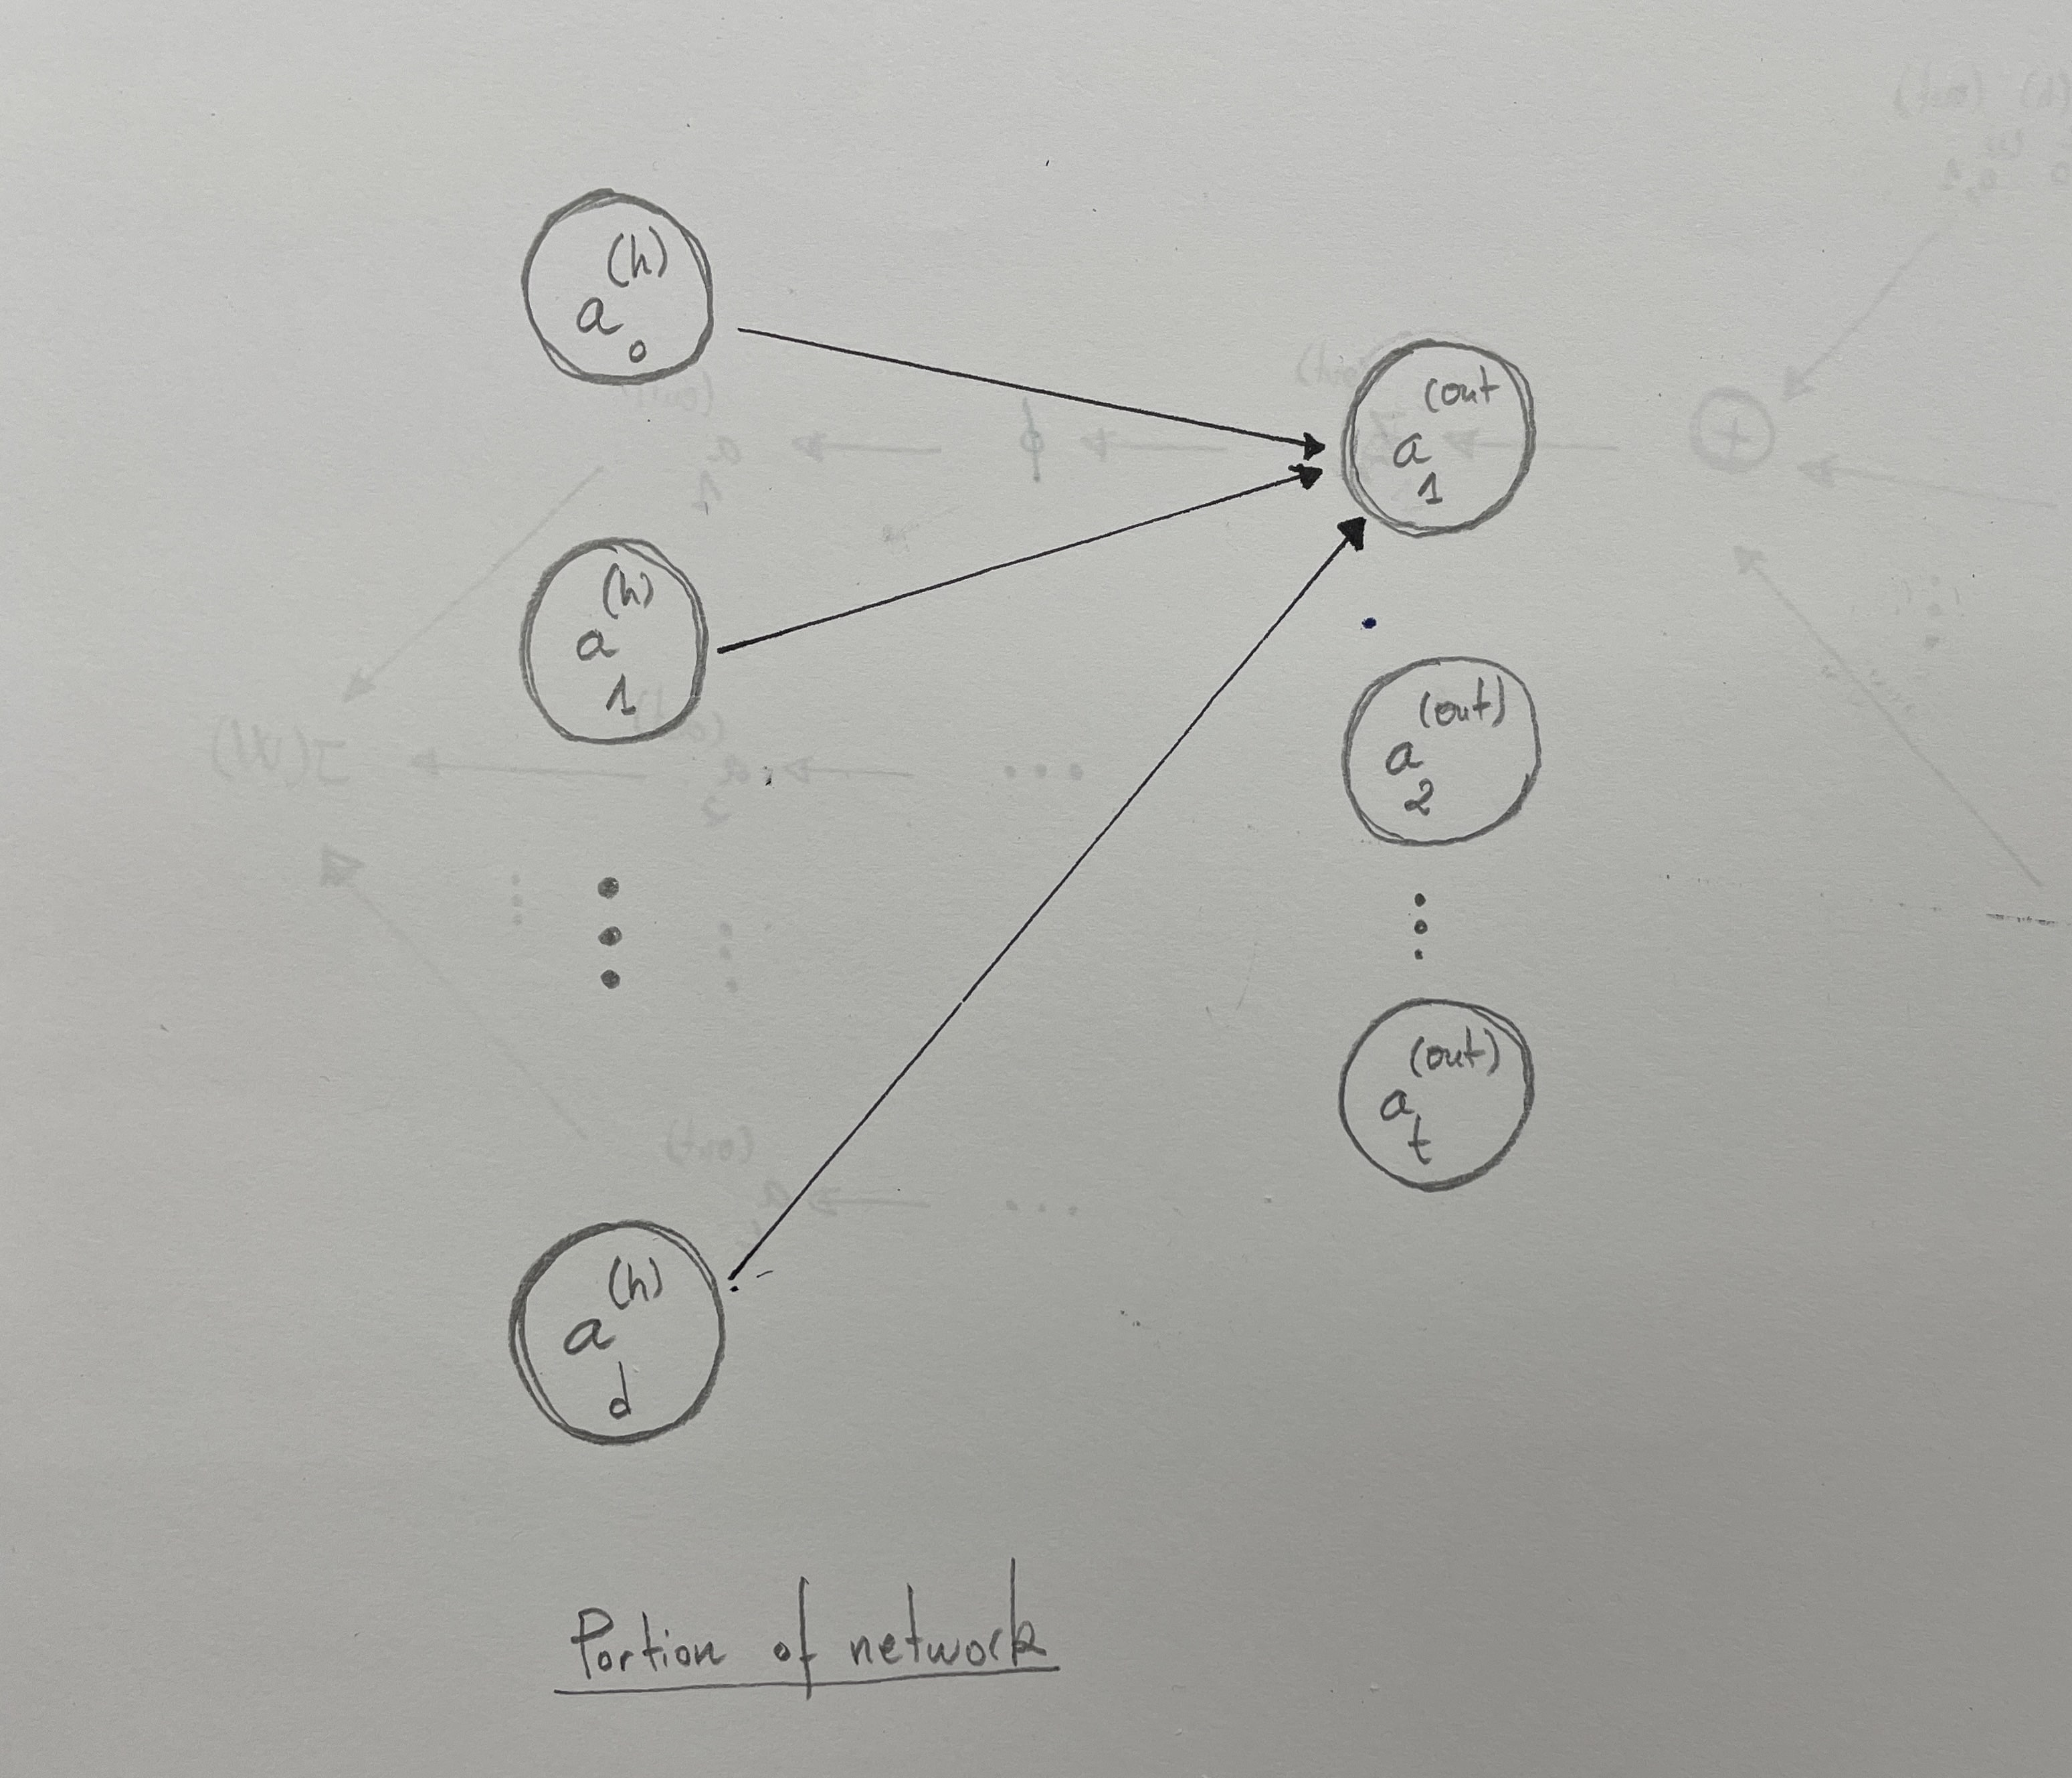
\includegraphics[width = 13cm, height = 12cm]{9.jpg}
\end{center}

\vspace{5mm} %5mm vertical space

The connections $w_{0,1}^{(out)}$, $w_{1,1}^{(out)}$, ..., $w_{d,1}^{(out)}$ are
highlighted in black this time. Again, let's look at them in detail:

\vspace{5mm} %5mm vertical space

%Portion of the network picture
\begin{center}
    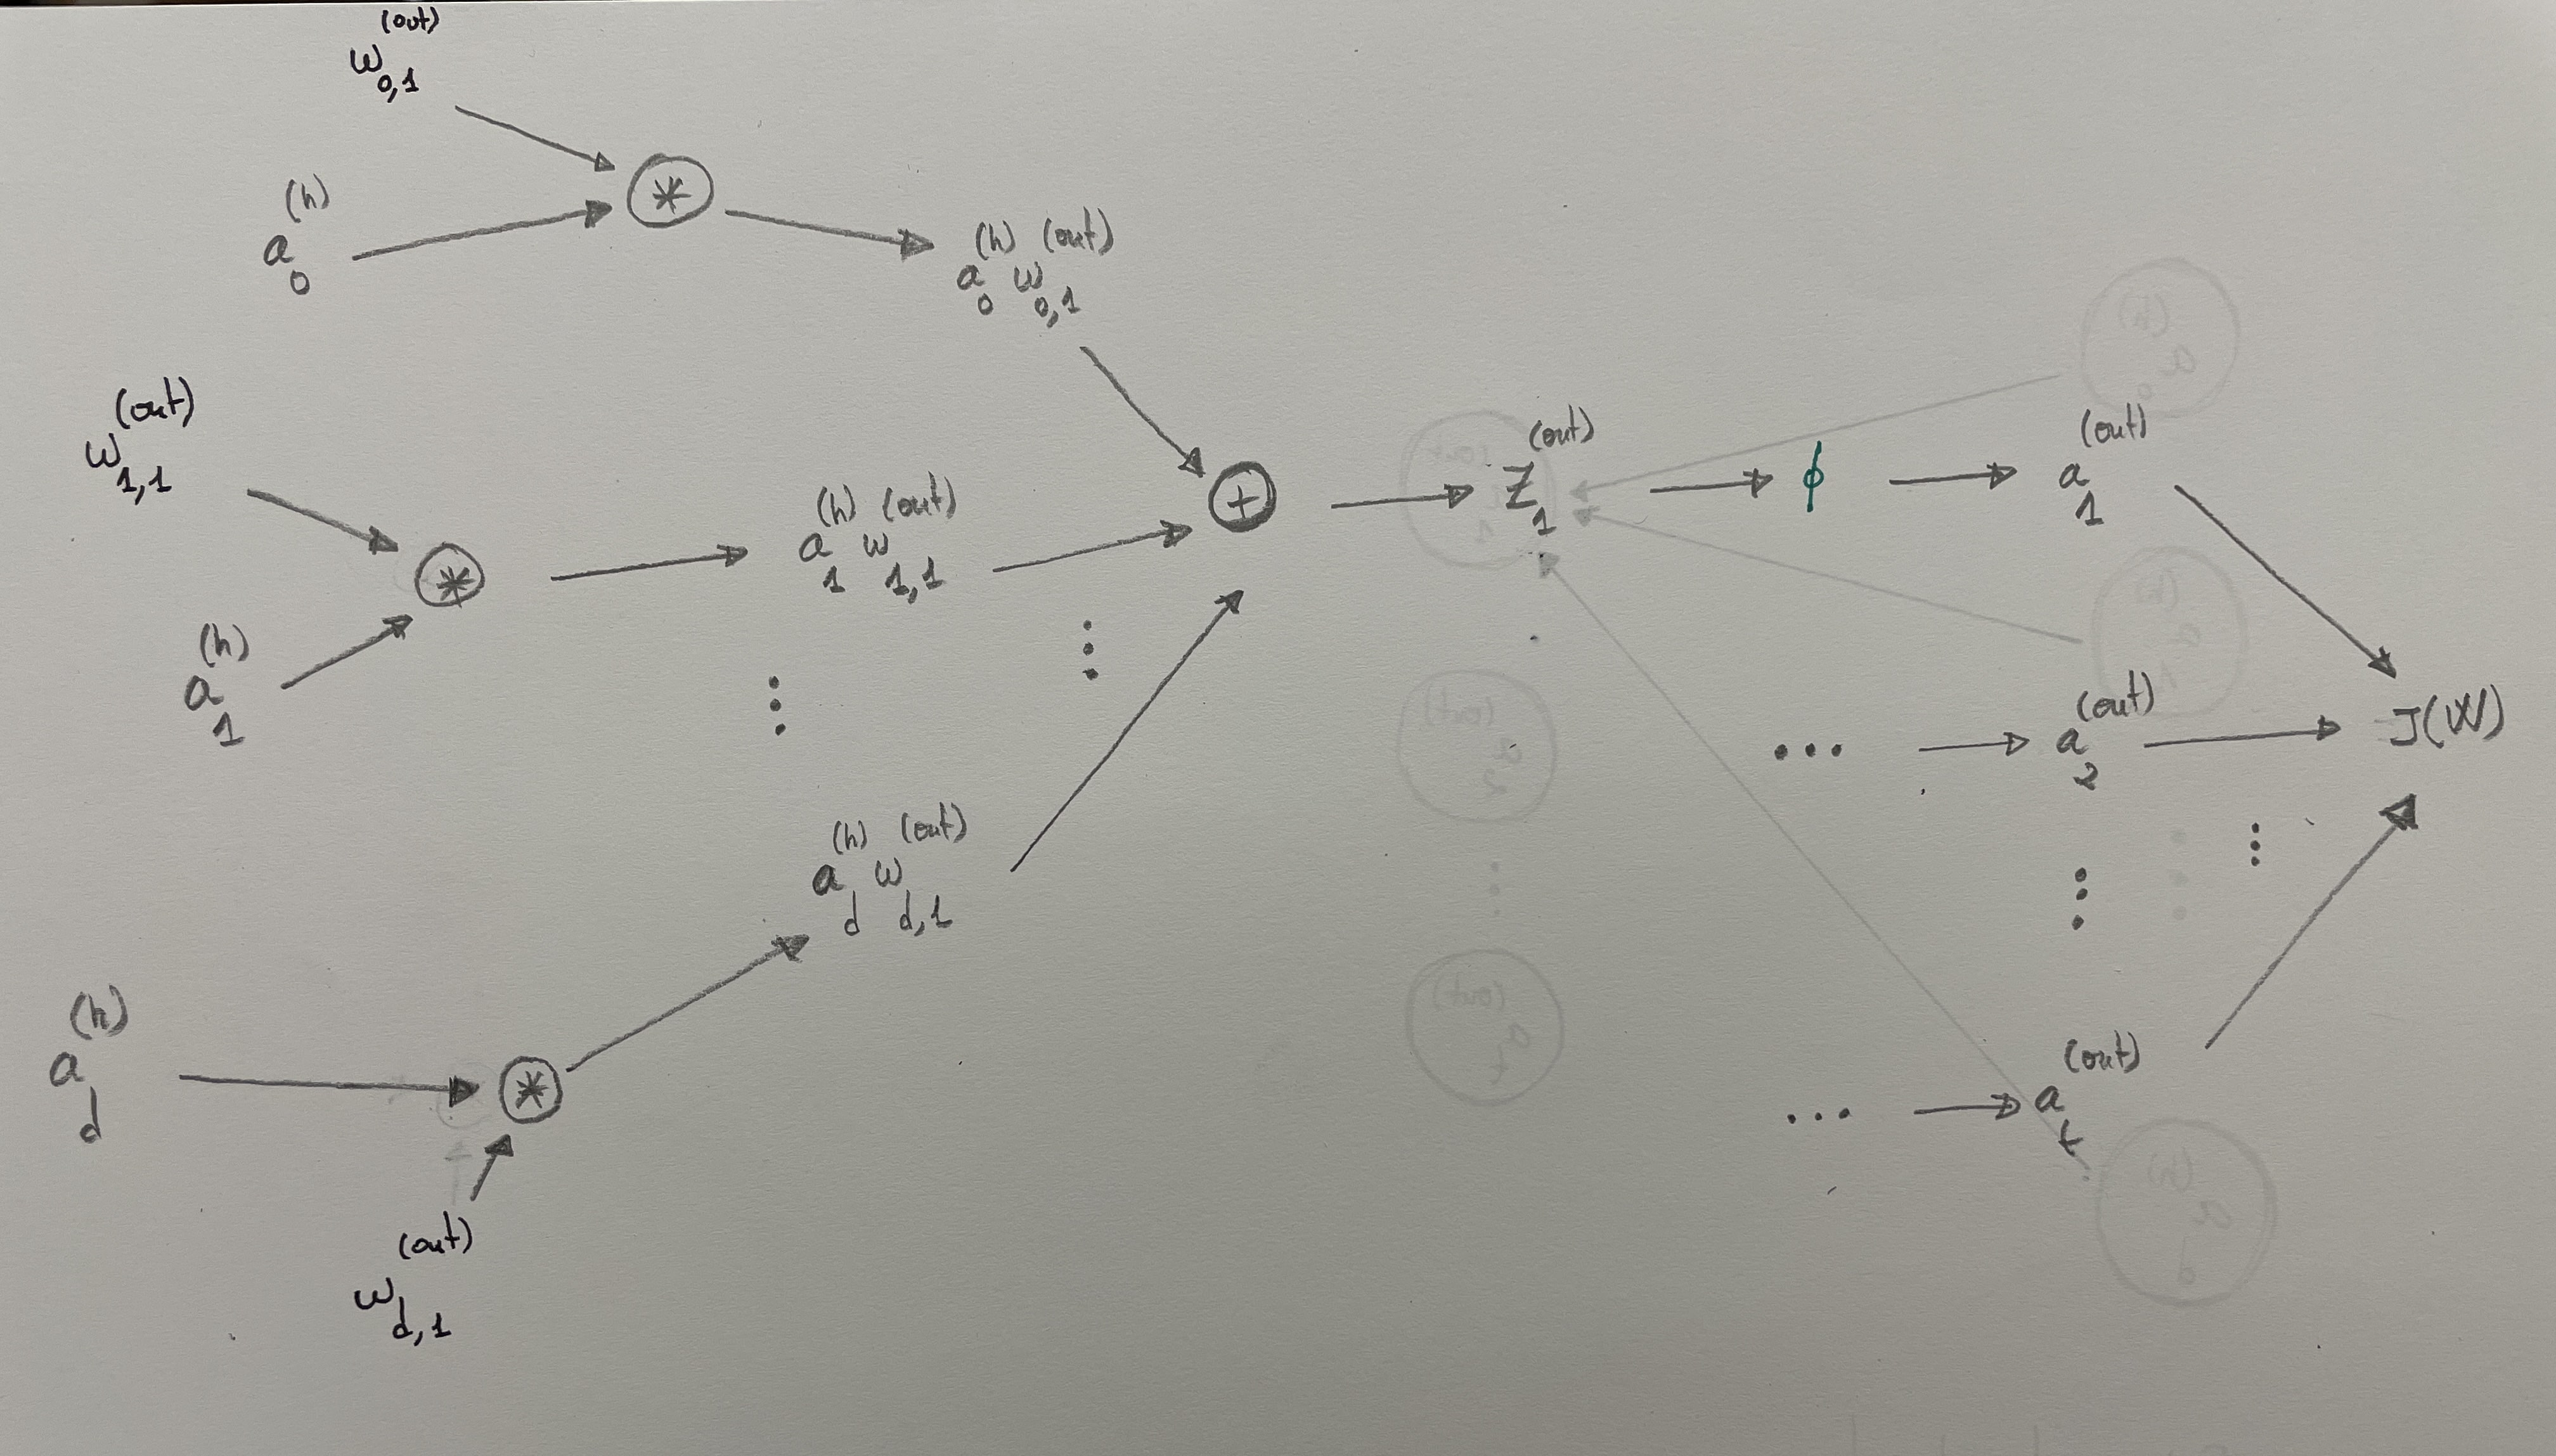
\includegraphics[width = 14cm, height = 9cm]{10.jpg}
\end{center}

\vspace{5mm} %5mm vertical space

Just like the previous times, let's compute the gradients one at time until
we find the gradients of the weights we are interested in. Let's start
with the loss value $J(W)$.

\vspace{5mm} %5mm vertical space

\[\frac{\partial J(W)}{\partial J(W)} = 1 \]

I continue with $a_{1}^{(out)}$

\[
    \frac{\partial J(W)}{\partial a_{1}^{(out)}} =
    \frac{a_{1}^{(out)} - y_{1}}{a_{{1}}^{(out)}(1 - a_{1}^{(out)})}
\]

\vspace{5mm} %5mm vertical space

Moving on with $z_{1}^{(out)}$

\[
    \frac{\partial J(W)}{\partial z_{1}^{(out)}} =
    \frac{\partial a_{1}^{(out)}}{\partial z_{1}^{(out)}} \times
    \frac{\partial J(W)}{\partial a_{1}^{(out)}} =
    a_{1}^{(out)}(1 - a_{1}^{(out)}) \bullet \frac{\partial J(W)}{\partial a_{1}^{(out)}} =
    a_{1}^{(out)} - y_1
\]

\vspace{5mm} %5mm vertical space

Let's continue with: $a_0^{(h)}w_{0,1}^{(out)}$, $a_1^{(h)}w_{1,1}^{(out)}$, ..., $a_d^{(h)}w_{d,1}^{(out)}$

\[
    \frac{\partial J(W)}{\partial a_0^{(h)}w_{0,1}^{(out)}} =
    \frac{\partial J(W)}{\partial a_1^{(h)}w_{1,1}^{(out)}} =
    \dots =
    \frac{\partial J(W)}{\partial a_d^{(h)}w_{d,1}^{(out)}} = 
    a_{1}^{(out)} - y_1
\]

\vspace{5mm} %5mm vertical space

The same gradients. Again.

\vspace{5mm} %5mm vertical space

Let's now determine the gradients of $w_{0,1}^{(out)}$, $w_{1,1}^{(out)}$, ..., $w_{d,1}^{(out)}$.
Here again, I will ignore the bias weight $w_{0,1}^{(out)}$, but will come back to it later.

\[
    \frac{\partial J(W)}{\partial w_{1,1}^{(out)}} =
    \frac{\partial a_1^{(h)}w_{1,1}^{(out)}}{\partial w_{1,1}^{(out)}} \times
    \frac{\partial J(W)}{\partial a_1^{(h)}w_{1,1}^{(out)}}  =
    a_1^{(h)}(a_{1}^{(out)} - y_{1})
\]

\[ \vdots \]

\[
    \frac{\partial J(W)}{\partial w_{d,1}^{(out)}} =
    \frac{\partial a_d^{(h)}w_{d,1}^{(out)}}{\partial w_{d,1}^{(out)}} \times
    \frac{\partial J(W)}{\partial a_d^{(h)}w_{d,1}^{(out)}}  =
    a_d^{(h)}(a_{1}^{(out)} - y_{1})
\]

\vspace{1cm} %1cm vertical space

Notice here again, how $a_{1}^{(out)} - y_{1}$ repeats in the results we found.
Let's call it $\delta_1^{(out)}$.

\vspace{1cm} %1cm vertical space

Using the chain rule, we computed the gradients of $w_{0,1}^{(out)}$, $w_{1,1}^{(out)}$, ..., $w_{d,1}^{(out)}$
starting with $J(W)$.
\end{document}